\documentclass[conference]{IEEEtran}
%\usepackage[cp1251]{inputenc}
%\usepackage{vmargin}
%\setpapersize{A4}
%\setmarginsrb{2cm}{1.5cm}{1cm}{1.5cm}{0pt}{0mm}{0pt}{13mm}
\usepackage{indentfirst}
\usepackage{amsmath}
\usepackage{amssymb}
\usepackage{mathrsfs}
\usepackage{amsthm}
\usepackage{graphicx}
\usepackage{tikz}
\usetikzlibrary{positioning}
\usetikzlibrary{decorations.fractals}
\usetikzlibrary{arrows,automata,decorations.markings}
%\usepackage{mathabx}
\usepackage{hyperref}

\newtheorem{theorem}{Theorem}
%\newtheorem{lemma}[theorem]{Lemma}
\newtheorem{corollary}{Corollary}
\sloppy

\begin{document}

\title{On the verification of strictly deterministic behaviour of Timed Finite State Machines}

\author
{
\IEEEauthorblockN{Evgenii Vinarskii}
\IEEEauthorblockA{\textit{Lomonosov Moscow State University} \\
Moscow, Russia \\
vinevg2015@gmail.com}
\and
\IEEEauthorblockN{ Vladimir Zakharov}
\IEEEauthorblockA{\textit{Lomonosov Moscow State University} \\
Moscow, Russia \\
zakh@cs.msu.su}
}

\maketitle

\begin{abstract}
	Finite State Machines (FSMs) are widely used as formal models for solving numerous tasks in software engineering, VLSI design, development of telecommunication systems, etc. To describe the behavior of a real-time system one could supply FSM model with clocks --- continuous time parameters with real values. In a Timed FSM (TFSM) inputs and outputs have timestamps, and each transition is equipped with a timed guard and an output delay to indicate time interval when the transition is active and how much time does it take to produce an output. A variety of algorithms for equivalence checking, minimization and test generation were developed for TFSMs in \cite{timed_fsm,timed_guard, tvar, zig}. A distinguishing feature of TFSMs studied in these papers is that the order in which outputs occure in an output timed word does not depend on their timestamps. We think that such behaviour of a TFSM is not realistic from the point of view of an outside observer. In this paper we consider a more advanced and adequate TFSM functioning; in our model the order in which outputs become visible to an outside observer is determined not only by the order of inputs, but also by delays required for their processing. When the same sequence of transitions is performed by a TFSM modified in a such way, the same outputs may follow in different order depending on the time when corresponding inputs become available to the machine. A TFSM is called strictly deterministic if for every sequence of transitions and for any input timed word which activates this sequence the letters in the output words always follows in the same order (but, maybe, with different timestamps). We studied the problem of checking whether a behaviour of an improved model of TFSM is strictly deterministic. To this end we showed how to verify whether an arbitrary given trace in a TFSM is strictly deterministic, and developed an exhaustive algorithm for checking the property of strict determinacy of TFSMs. Exhaustive search in this case can hardly be avoided: we proved that determinacy checking problem for our model of TFSM is co-NP-hard.
\end{abstract}

\section{Introduction}

Finite State Machines (FSMs) are widely used as formal models for analysis and synthesis of information processing systems in software engineering, VLSI design, telecommunication, etc. The most attractive feature of this model of computation is its simplicity --- many important synthesis and analysis problems (equivalence checking, minimization, test derivation, etc.) for classical FSMs can be solved in time which is almost linear or quadratic of the size of a FSM under consideration. 

The concept of FSM is rather flexible. Since in many applications time aspects such as durations, delays, timeouts are very important, FSMs can be augmented with some additional features to describe the dependence of the behavior of a system on events occurring in real time. One of the most advanced timed extension of FSMs is the concept of Timed Automata which was developed and studied in \cite{alur}. Timed Automata are supplied with clocks (timers) for indicating real time moments, measuring durations of events, providing timeout effects. Transitions in such automata depend not only on the incoming of the outside messages and signals but also on the values of clocks. Further research showed that this model of computation is very expressive and captures many important features of real-time systems behaviour. On the other side, Timed Automata in the full scope of their computing power are very hard for analysis and transformations (see \cite{alur2,finkel}). 

When a Timed Automaton is capable to selectively reset timers it can display rather sophisticated behaviour which is very difficult for understanding and analysis. In some cases such ability is very important; see, e.g.~\cite{fletcher}. But a great deal of real-time programs and devices operate with timers much more simply: as soon as such a device switches to a new mode of operation (new state), it resets all timers. Timed Finite State Machines (TFSMs) of this kind were studied in \cite{timed_fsm, merayo, timed_guard, tvar}. TFSM has the only timer which it resets "automatically'' as soon as it moves from one state to another. On the other hand, TFSMs, in contrast to Timed Automata introduced in \cite{alur}, operate like transducers: they receive a sequence of input signals augmented with their timestamps (input timed word) and output a sequence of responses also labeled by timestamps (output timed word). The timestamps are real numbers which indicate the time when input signals become available to TFSM or output responses are generated. Transitions of TFSMs are equipped with time guards to indicate time intervals when transitions are active. Therefore, a reaction of a TFSM to an input signal depends not only on the signal itself but also on its timestamp. Some algorithms for equivalence checking, minimization and test generation were developed for TFSMs in \cite{timed_fsm,timed_guard, tvar, zig}. It can be recognized that this model of TFSM combines a sufficient expressive power for modeling a wide class of real-time information processing systems and algorithmic support.   

As it was noticed above a behaviour of a TFSM is characterized by a paired sequences: an input timed word and a corresponding output timed word. A distinguishing feature of TFSMs studied in \cite{timed_fsm, merayo, timed_guard, tvar, zig} is that an output timed word is formed of timestamped output letters that follows in the same order as the corresponding input letters regardless of their timestamps. Meanwhile, suppose that a user of some file management system gives a command "Save'' and immediately after that a command "Exit''. Then if a file to be saved is small then the user will observe first a response "File is saved'' and then a notification "File Management System is closed''. But if a file has a considerable size then it takes a lot of time to close it. Therefore, it can happen that a user will detect  first a notification "File Management System is closed'' and then, some time later, he/she will be surprised to find an announcement "File  is saved''. Of course, the user may regard such behaviour of the system enigmatic. But much worse if the order in which these notifications appear may vary in different sessions of the system. If a File Management System interacts with other service programs such behaviour will almost certainly lead to errors. However, if TFSM is defined as in the papers referred above then such a model can not adequately capture behavioral defects of real-time systems, similar to the one that was considered in the example.   

To avoid this shortcoming of conventional TFSMs and to make their behaviour more "realistic'' from the point of view of an outside observer we offer some technical change to this model. We will assume that an output timed word consists of timestamped letters, and these letters always follow in ascending order of their timestamps regardless of an order in which the corresponding input letters entered a TFSM. In this model an input $b$ may follow an input $a$ but a response to $b$ may appear before a response to $a$ is computed. Clearly, the defect with File Management System discussed above becomes visible to an outside observer "through'' the model of TFSMs thus modified. 

At first sight, it may seem that this change slightly complicates the analysis of the behavior of such models. But this is a false impression. In the initial model of TFSM the formation of an output timed word is carried out by local means for each state of the system. In our model this is a global task since to find the proper position of a timestamped output letter one should consider the run of TFSM as a whole. Therefore, even the problem of checking whether a behaviour of an improved model of TFSM is deterministic can not be solved as easy and straightforwardly as in the case of initial model of TFSM. 

We studied determinacy checking problem for improved TFSMs and present the results of our research in this paper. First, we offer a criterion to determine whether a given trace in a TFSM is strictly deterministic, i.e. for any input timed word which activates this trace the letters of output words always follow in the same order (but, maybe, with different timestamps). Then, using this criterion we developed an exhaustive algorithm for checking the property of strict determinacy of TFSMs. Exhaustive search, although been time consuming, can hardly be avoided in this case: we proved that determinacy checking problem for improved version of TFSMs is co-NP-complete by polynomially reducing to its complement the subset-sum problem \cite{ssp} which is known to be NP-hard.

The structure of the paper is as follows. In Section 2 we define the basic notions and introduce an improved concept of TFSM (or, it would be better said, a concept of TFSM with an improved behaviour). In Section 3 we present necessary and sufficient conditions for strict determinism of traces in a TFSM. In Section 4 we discuss how to use this criterion to check whether a given TFSM is strictly deterministic. Section 5 contains the results on the complexity of checking the properties of strictly deterministic behavior of TFSM. In the Conclusion we breifly outline the consequences of our results and topics for further research.


\section{Preliminaries}

Consider two non-empty finite alphabets $I$ and $O$; the alphabet $I$ is an \emph{input alphabet} and the alphabet $O$ is an \emph{output alphabet}. The letters from $I$ can be regarded as control signals received by some real-time computing system, whereas the letters from $O$ may be viewed as responses (actions) generated by the system. A finite sequence $w = i_1, i_2, \dots, i_n$  of input letters is called an \emph{ input word}, whereas a sequence $z = o_1, o_2, \dots, o_n$ of output letters is called an \emph{output word}.
As usual, the time domain is represented by the set of non-negative reals $\mathbb{R}_0^+$. The set of all positive real numbers will be denoted by $\mathbb{R}^+$. When such a system receives a control signal (a letter $i$) its output depends not only on the input signal $i$ itself but also on
\begin{itemize}
	\item a current internal state of the system,
	\item a time instance when $i$ becomes available to a system, and
	\item time required to process the input (output delay).
\end{itemize}
These aspects of real-time behaviour can be formalized with the help of timestamps, time guards and delays. A timestamp as well as a delay is a real number from $\mathbb{R}^{+}$. A \emph{timestamp} indicates a time instance when the system receives an input signal or generates a response to it. A \emph{delay} is time the system needs to generate an output response after receiving an input signal. A \emph{time guard} is an interval $g = \langle u, v \rangle$, where $\langle \in \{ (, [ \}$, $\rangle \in \{ ), ] \}$, and $u, v$ are timestamps such that $0 < u < v$. Time intervals indicate the periods of time when transitions of a system are active for processing input signals. As usual, the term \emph{time sequences} is reserved for an increasing sequence of timestamp. For the sake of simplisity we will deal in follows only with time guards of the form $(u,v]$: the result obtained can be adapted with minor changes to arbitrary time guards. 

Let $w = x_1, x_2, \dots x_n$ and $\tau = t_1, t_2, \dots, t_n$ be an input (output) word and a time sequence, respectively, of the same length. Then a pair $(w, \tau )$ is called a \emph{timed word}. Every pair of corresponding elements $x_j$ and $t_j$, $1\leq j \leq n,$  indicates that an input signal (or an output response) $x_j$ appears at time instance $t_j$. In order to make this correspondence more clear we will write sometime timed words as sequences of pairs $(w, \tau ) = (i_1, t_1), (i_2, t_2), \dots, (i_n, t_n)$  whose components are input signals (or output responses) and their timestamps.   
 
A \emph{Finite State Machine} (\emph{FSM}) over the alphabets $I$ and $O$ is a triple $M = \langle S, s_0, \rho \rangle$ where 
\begin{itemize}
\item
$S$ is a finite non-empty set of \emph{states},
\item
$s_0$ is an \emph{initial state},
\item
$\rho \subseteq (S \times I \times O \times S)$ is a \emph{transition} relation. 
\end{itemize}
A transition $(s, i, o, s')$ means that FSM $M$ when being at the state $s$ and receiving an input signal $i$ passes its control (moves) to the state $s'$ and generates the output response $o$.

%An FSM is \emph{complete} if for every pair $(s, i) \in S \times I$ there exists a transition $(s, i, o, s^{\prime}) \in h_S$, otherwise it is \emph{partial}. An FSM is \emph{deterministic} if for every pair $(s, i) \in S \times I$ there exists at most one transition $(s, i, o, s^{\prime}) \in h_S$, otherwise it is called \emph{non-deterministic}.

FSMs can not measure time and, therefore, they are not adapted to model the behavior of real-time systems. The authors of \cite{alur} proposed to equip  FSMs with clocks --- variables which take non-negative real values. To manipulate with clocks machines use reset instructions, timed guards and output delays. Time guards indicate time intervals during which transitions are active and input signals can be processed. An output delay indicates how much time does it take to process an input. Thus, every transition in such a machine is a quadruple $\langle\textit{input, timed guard, output, delay}\rangle$. Input signals and output responses are accompanied by timestamps. If an \emph{input} is marked by a timestamp which satisfies the \emph{time guard} then the transition fires, the machine moves to the next state and generates the \emph{output}. This output is marked by a timestamp which is equal to the timestamp of the input plus the \emph{delay}. For real-time machines of this kind usual problems from automata theory (equivalence and containment checking, minimization, etc.) may be set up and solved. Minimization problem for real-time machines is very important, since the complexity of many problems of analysis and synthesis depends on the size of machines. In \cite{tvar} this problem was studied under the so called "slow environment assumption'': next input becomes available only after an output response to the previous one is generated. In this paper, we consider a more advanced real-time machine; in this model the order in which outputs become visible to an outside observer is determined not only by the order in which inputs follow, but also by the delay required for their processing. When the same sequence of transitions is performed by such a machine the same outputs may follow in different order depending on the arriving time of the corresponding inputs. Our ultimate aim is to develop a minimization algorithms for real-time machines of this kind. But, as in the case of Finite State Automata, minimization problem may have efficient solution only for deterministic machines. Thus, our first step toward the solution of minimization problem is to find a way to check if the behaviour of a machine is deterministic.

Formally, by Timed FSM (TFSM) over the alphabets $I$ and $O$ we mean a quadruple \bf $M = $ \normalfont $( S, s_{in}, G, \rho )$ where:
\begin{itemize}
	\item $S$ is a finite non-empty \emph{set of states},
	\item $s_{in}$ is \emph{an initial state}.
	\item $G$ is a set of \emph{timed guards},
	\item $\rho \subseteq (S \times I \times  O \times S \times G \times \mathbb{R}^+)$ is a \emph{transition relation}.
\end{itemize}
A transition $(s, i, o, s', g, d)$ should be understood as follows: the TFSM when being at the state $s$ and receiving the the input letter $i$ marked by a such timestamp $t$ that $t \in g $ moves to the state $ s' $ and outputs the letter $o$ marked with the timestamp $\tau=t+ d$. When algorithmic and complexity issues of TFSM's analysis and synthesis are concerned then we assume that time guards and delays are rational numbers, and the size of a TFSM is the length of a binary string which encodes all transitions in the TFSM.

A \emph{trace} in TFSM $M$ is any sequence of transitions $ (s_0, a_1, b_1, s_1 (u_1, v_1], d_1), \dots,(s_{n-1}, a_n, b_n, s_n, (u_n, v_n ], d_n) $, where every state $s_j$, $0< j <n$, is an arrival state of one transition and a departure state of the next transition. The trace $tr$ \emph{converts} an input timed word $\alpha = (a_1, t_1), (a_2, t_2), \dots, (a_n, t_n)$ to the timed output word $\beta=(b_{j_1},\tau_1),(b_{j_2},\tau_2),\dots,(b_{j_n},\tau_n)$, iff
\begin{itemize}
	\item $t_j - t_{j-1}\in (u_j,v_j]$ holds for all $j, 1\leq i\leq n$ (it is assumed that $t_0=0$);
	\item $\beta$ is such a permutation of the sequence $ \gamma = (b_1, t_1 + d_1), (b_2, t_2 + d_2), \dots, (b_n, t_n + d_n) $ that the second components of the pairs $\tau_1,\tau_2,\dots,\tau_n$ constitute a time sequence.
\end{itemize}
Clearly, for every trace $tr$ and an input timed word $\alpha$ its conversion $\beta$ (if any) is determined uniquely; such a conversion will be denoted as $conv(tr,\alpha)$. If $conv(tr,\alpha)$ is defined then we say that the input timed word $\alpha$ \emph{activates} the trace $tr$. We will say that the output word $b_{j_1}, b_{j_2}, \dots, b_{j_n}$ is a \emph{plain response} to the input timed word $\alpha$ on the trace $tr$; it will be denoted as $resp(tr,\alpha)$.

%\begin{figure}
%	\begin{center}
%		\includegraphics[width=0.4\textwidth]{counterExample.pdf}
%		\caption{TFSM \bf $ M $ \normalfont}
%	\end{center}
%\end{figure}

\noindent
\fbox
{
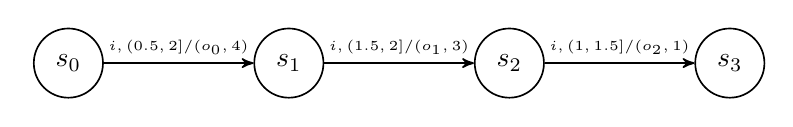
\begin{tikzpicture}[>=stealth',node distance=2.8cm,semithick,auto,scale=0.3, every node/.style={scale=1}]
				\node[state]	    (0)	{$s_0$};
				\node[right of=0, state]	(1) {$s_1$};
				\node[right of=1, state]	(2) {$s_2$};
				\node[right of=2, state]	(3) {$s_3$};

				\begin{scope}[node distance=0.4cm]
				\node	[right of=1] (s3) {};
				\node	[left of=0] (s4) {};
				\end{scope}
				{
				\scriptsize
				\path[->] 
				(0) edge [midway] node{\tiny $ i, (0.5, 2]/(o_0, 4) $ \normalsize} (1)

				(1) edge [midway] node{\tiny $ i, (1.5, 2]/(o_1, 3) $ \normalsize} (2)

				(2) edge [midway] node{\tiny $ i, (1, 1.5]/(o_2, 1) $ \normalsize} (3)

					;
				}
\end{tikzpicture}
}
\begin{center}
	\begin{small}
		Fig.1 TFSM $M$
	\end{small}
\end{center}

Consider, for example, a TFSM $M$ depicted in Fig. 1 and a trace
$$
(s_0, i, s_1, o_0, (0.5, 2], 4), (s_1, i, s_2, o_1, (1.5, 2], 3), (s_2, i, s_3, o_2, (1, 1.5], 1)
$$
in this TFSM. Then this trace

\begin{enumerate}
	\item accepts an input timed word $\alpha_1=(i, 1),(i, 2.7),(i, 4.1)$ and converts it to the output timed word 
	$\beta_1=(o_1, 5),(o_3, 5.1),(0_2, 5.7) $; thus, the plain response of $M$ to $\alpha_1$ is $w_1=o_1, o_3, o_2 $;
	\item accepts an input timed word $\alpha_2=(i, 1.5),(i, 3.2),(i, 4.3)$ and converts it to the output timed word 
	$\beta_2=(o_3, 5.3),(o_1, 5.5),(o_2, 6.2) $, and the plain response of $M$ to $\alpha_2$ is $w_2=o_3, o_1, o_2 $ which is different from $w_1$;
	\item does not accept an input timed word $\alpha_3=(i, 2.3),(i, 4),(i, 6)$.
\end{enumerate}

\section{Strictly deterministic traces and TFSMs}

As can be seen from the above example, a pair of input timed words that differ only in timestamps of input signals may activate the same trace in a TFSM, although plain responses of TFSM to these words are different. Generally speaking, there is nothing unusual in this: in real-time models not only the input signals, but also the values of timers influence a run of a model. Nevertheless, in many applications it is critically important to be sure that the behaviour of a real-time system is predictable: once a system choose a mode of computation (i.e. a trace in TFSM) it will behave in a similar way (i.e. give the same plain response) in all computations of this mode. Traditionally, computer systems in which for any input data the processing mode is uniquely determined by the system are called deterministic. But for our model of real-time systems this requirement should be clarified and strengthened. For this purpose we introduce the property of strict determinacy of a real-time system. 

A trace $tr$ in TFSM $M$ is called \emph{strictly deterministic} if $resp(tr,\alpha_1)=resp(tr,\alpha_2)$ holds for every pair of input timed words $\alpha_1$ and $\alpha_2$ that activate $tr$. A TFSM $M=( S, s_{in}, G, \rho)$ is called \emph{deterministic} iff for every pair of transitions $(s,i_1,o_1,s',(u_1,v_1], d_1)$ and $(s,i_2,o_2,s'',(u_2,v_2], d_2)$ in $\rho$ either $i_1\ne i_2$, or $(u_1,v_1] \cap (u_2,v_2]=\emptyset$. This requirement means that every timestamped input letter can activate no more than one transition from an arbitrary given state $s$. It also implies that every input timed word can activate no more than one trace in $M$. A deterministic TFSM is called strictly deterministic iff every initial trace in $M$ which starts from the initial state $s_{in}$ is strictly deterministic. It is easy to see that TFSM, depicted in Fig. 1, is not strictly deterministic. 

The Strict Determinacy Checking Problem (in what follows, SDCP) is that of checking, given a TFSM or a trace in a TFSM, if it is strictly deterministic. It should be noticed that SDCP can not be solved by local means only, i.e. by considering one by one all states of a TFSM in the same way as to check that a TFSM is deterministic in the usual sense of this term. A simple criterion for strict determinacy of traces is presented as a Theorem below.

%%%%%%%%%%%%%%%%%%%%%%%%%%

Let a sequence of transitions
$$
(s_0, i_1, s_1, o_1, \langle u_1, v_1 \rangle, d_1), \dots, (s_{n - 1}, i_n, s_n, o_n, \langle u_n, v_n \rangle, d_n)
$$
be a trace $tr$ in a TFSM $M$.
Then the following theorem holds.

\begin{theorem}
{\itshape
A trace $tr$ is strictly deterministic if and only if for all pairs of integers $k, m$ such that $1 \leq k < m \leq n$ at least one of the two inequalities $d_k - d_m \leq \sum\limits_{j = k + 1}^{m}u_j$ or $d_k - d_m > \sum\limits_{j = k + 1}^{m}v_j$ hold.
}
\end{theorem}
\begin{proof}

($\Rightarrow$) Suppose that there exists a pair $k, m$ such that $1 \leq k < m \leq n$, and a double inequality holds:
$$
\sum\limits_{j = k + 1}^{m}u_j < d_k - d_m \leq \sum\limits_{j = k + 1}^{m}v_j \ .
$$
Then we use two positive numbers $r = d_k - d_m - \sum\limits_{j = k + 1}^{m}u_j$ and $\varepsilon = \frac{r}{n}$ and consider a behaviour of a TFSM $M$ in the input timed words
$$
\begin{array}{l}
\alpha' = (i_1, v_1), \dots, (i_k, v_k), (i_{k + 1}, u_{k + 1}\!+\!\varepsilon),\!\dots,\!(i_m, u_m\!+\!\varepsilon),\\
\alpha'' = (i_1, v_1), \dots, (i_k, v_k), (i_{k + 1}, v_{k + 1}), \dots, (i_m, v_m).
\end{array}
$$
It is easy to see that both words activate $tr$. 

The trace $tr$ converts the timed input word $\alpha_1$ to the timed output word  
$$
conv(tr,\alpha')= \dots, (o_m, T'_m), \dots, (o_k, T'_k), \dots
$$
such that $T'_m = \sum\limits_{j = 1}^{k}v_j + \sum\limits_{j = k + 1}^{m}(u_j + \varepsilon) + d_m$, and $T'_k = \sum\limits_{j = 1}^{k}v_j + d_k$. In this timed output word, the output letter $o_k$ follows the output letter $o_m$ since
$$
T'_k - T'_m = d_k - d_m - \sum\limits_{j = k + 1}^{m}u_j + (m - k)\varepsilon = r - \frac{r(m - k)}{n} > 0.
$$
Hence, $resp(tr, \alpha') = \dots, o_m, \dots, o_k, \dots$.

 On the other hand, the trace $tr$ converts the timed input word $\alpha''$ to the timed output word
$$
conv(tr,\alpha'')= \dots, (o_k, T''_k), \dots, (o_m, T''_m), \dots
$$
such that $T''_k = \sum\limits_{j = 1}^{k}v_j + d_k$ and $T''_m = \sum\limits_{j = 1}^{m}v_j + d_m$. In this timed output word the output letter $o_m$ follows the output letter $o_k$ since
$$
T''_m - T''_k = d_m - d_k = \sum\limits_{j = k + 1}^{m}v_j \geq 0
$$
Therefore, $resp(tr, \alpha'') = \dots, o_k, \dots, o_m, \dots$.

Thus, we got evidence that the trace $tr$ is not strictly deterministic.
\smallskip

\noindent
($\Leftarrow$) Suppose that the trace $tr$ is not strictly deterministic. Then there exists a pair of timed input words $\alpha' = (i_1, t'_1), \dots, (i_n, t'_n)$ and $\alpha'' = (i_1, t''_1), \dots, (i_n, t''_n)$ such that both words activate the trace $tr$ and $resp(tr, \alpha') \neq resp(tr, \alpha'')$. Consequently, there exists a pair of output letters $o_m$ and $o_k$ such that 
$$\begin{array}{l}
conv(tr, \alpha') = \dots, (o_k, T'_k), \dots, (o_m, T'_m), \dots\\
conv(tr, \alpha'') = \dots, (o_m, T''_m), \dots, (o_k, T''_k), \dots \ .
\end{array}
$$ 
Such permutation of output letters is possible iff the following inequalities hold  
$$
\begin{array}{l}
t'_k + d_k = T'_k < T'_m=t'_m + d_m ,\\
t''_k + d_k = T''_k > T''_m=t''_m + d_m  \ .
\end{array}
$$
But since both input timed words $\alpha'$ and $\alpha''$ activate $tr$, we have the following chain of inequalities: \\
$$
\sum\limits_{j = k + 1}^{m}u_j < T''_m - T''_k < d_k - d_m < T'_m - T'_k \leq \sum\limits_{j = k + 1}^{m}v_j.
$$
Thus, if $tr$ is not strictly deterministic then there exists a pair of integers such that $1 \leq k < m \leq n$ and 
$$
\sum\limits_{j = k + 1}^{m}u_j < d_k - d_m \leq \sum\limits_{j = k + 1}^{m}v_j 
$$
holds.
\end{proof}

%%%%%%%%%%%%%%%%%%%%%%%%%%

Now, having the criterion for strict determinacy of traces, we can give a solution to SDCP for TFSMs. Let TFSM $M = (S, s_{in}, G, \rho)$ be a deterministic TFSM. Denote by $u_{min}$ the greatest lower bound of all left boundaries used in the time guards of $M$. In our model of TFSM $u_{min}\ne 0$. let $d_{min}$ and $d_{max}$ be the minimum and the maximum output delays occurred in the transitions of $M$. A theorem below gives necessary and sufficient conditions for the behaviour of $M$ to be strictly deterministic.

\begin{theorem}
{\itshape
A deterministic TFSM $M$ is strictly deterministic iff all its traces of length $p$, where $p = \lceil \frac{d_{max} - d_{min}}{u_{min}} \rceil$, are strictly deterministic.
}
\end{theorem}
\begin{proof}
	The necessity of conditions is obvious.
	
	We prove the sufficiency of conditions by contradiction. Suppose that all traces of length less or equal $p$ are strictly deterministic but TFSM $M$ is not. Then there exists such a trace $tr$ in $M$ which is not strictly deterministic. Then, by Theorem 1, this trace is a sequence of transitions $(s_{j-1}, i_j, s_j, b_j, (u_j, v_j], d_j), 1\leq j\leq n$, such that for some pair of integers $m$ and $k$, where $1 \leq k < m \leq n$, two inequalities 
$$ 
\sum\limits_{j = k + 1}^{m}u_j \leq d_k - d_m \leq \sum\limits_{j = k + 1}^{m} v_j 
$$ 
hold. It should be noticed, that, by the same Theorem 1, the trace $tr'$ which includes only the transitions $(s_{j-1}, i_j, s_j, b_j, (u_j, v_j], d_j), m\leq j\leq k$, is not strictly deterministic as well. Hence, $ m - k > p $, and we have the following sequence of inequalities
$$ 
d_{max} - d_{min} \geq d_m - d_k \geq \sum_{j = k + 1}^{m}u_j > p * u_{min} 
$$
which contradicts our choice of $p = \lceil \frac{d_{max} - d_{min}}{u_{min}} \rceil $.
\end{proof}

As it follows from Theorems 1 and 2, to guarantee that a given TFSM $M = (S, s_{in}, G, \rho )$ is strictly deterministic it is sufficient to consider all traces $(s_0, a_1, b_1, s_1, (u_1, v_1], d_1), \dots,(s_{n-1}, a_n, b_n, s_n, (u_n, v_n], d_n)$ in $M$, whose length $n$ does not exceed the value $p = \lceil \frac{d_{max} - d_{min}}{u_{min}} \rceil$ defined in Theorem 2, and for every such trace check that one of the inequalities $d_1 - d_n < \sum\limits_{j = 2}^{n}u_j$ or $d_1 - d_n > \sum\limits_{j = 2}^{n}v_j$ holds. Thus, we arrive at

\begin{corollary}
{\itshape
SDCP for TFSMs is decidable.
}
\end{corollary}

%\begin{figure}
%	\begin{center}
%		\includegraphics[width=0.4\textwidth]{fsm_np.pdf}
%		\caption{TFSM \bf $ M $ \normalfont}
%	\end{center}
%\end{figure}

\noindent
\fbox
{
\tikzstyle{vecArrow} = [thick, decoration={markings,mark=at position
   1 with {\arrow[semithick]{open triangle 60}}},
   double distance=1.4pt, shorten >= 5.5pt,
   preaction = {decorate},
   postaction = {draw,line width=1.4pt, white,shorten >= 4.5pt}]
\tikzstyle{innerWhite} = [semithick, white,line width=1.4pt, shorten >= 4.5pt]
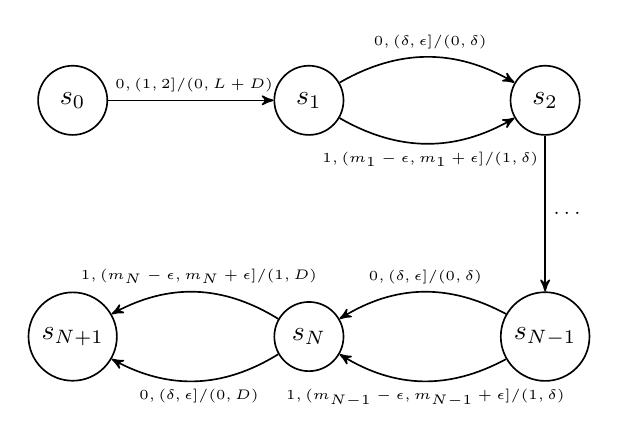
\begin{tikzpicture}[>=stealth',node distance=3cm,semithick,auto,scale=0.5, every node/.style={scale=1}]
				\node[state]	(0)	{$s_0$};
				\node[right of=0, state]	(1) {$s_1$};
				\node[right of=1, state]	(2) {$s_2$};
				\node[below of=2, state]	(3) {$s_{N - 1}$};
				\node[below of=1, state]	(4) {$s_{N}$};
				\node[below of=0, state]	(5) {$s_{N + 1}$};
				
				{\scriptsize
				\path[->] 
				(0) edge [midway] node{\begin{tiny} $0, (1, 2] / (0, L + D)$ \end{tiny}} (1)

				(1) edge [above, bend left] node{\begin{tiny} $0, (\delta, \epsilon] / (0, \delta)$ \end{tiny}} (2)
					  edge [below, bend right] node{\begin{tiny} $1, (m_1 - \epsilon, m_1 + \epsilon] / (1, \delta)$ \end{tiny}} (2)
				
				(2) edge [midway] node{$\dots$} (3)
				
				(3) edge [above, bend right] node{\begin{tiny} $0, (\delta, \epsilon] / (0, \delta)$ \end{tiny}} (4)
					  edge [below, bend left] node{\begin{tiny} $1, (m_{N - 1} - \epsilon, m_{N - 1} + \epsilon] / (1, \delta)$ \end{tiny}} (4)
				
				(4) edge [below, bend left] node{\begin{tiny} $0, (\delta, \epsilon] / (0, D)$ \end{tiny}} (5)
					  edge [above, bend right] node{\begin{tiny} $1, (m_{N} - \epsilon, m_{N} + \epsilon] / (1, D)$ \end{tiny}} (5)
					;
				}
\end{tikzpicture}
}
\begin{center}
	\begin{small}
		Fig.2 TFSM $M$
	\end{small}
\end{center}

\section{SDCP is co-NP-hard}

Clearly, the decision procedure, based on Theorem 2, is time consuming since $p$ may be exponential of the size of $M$ and the number of traces of length $p$ in TFSM $M$ is exponential of $p$. In this section we show that such an exhaustive search can hardly be avoided because SDCP for improved version of TFSMs is co-NP-hard. 

We are aimed to show that the complement of SDCP is NP-hard. To this end we consider the Subset-Sum Problem (see \cite{ssp}) which is known to be NP-complete and demonstrate that this problem can be polynomially reduced to the complement of SDCP for TFSMs. 

The Subset-Sum Problem (SSP) is that of checking, given a set of integers $Q$ and an integer $L$, is there any subset $Q', Q'\subseteq Q$, such that the sum of all its elements is equal to $L$. More formally, the variant of the SSP we are interested in is defined as follows. Let $Q=m_1,m_2,\dots, m_N$ be a sequence of positive integers, and $L$ be also a positive integer. A solution to $(Q,L)$-instance of SSP is a binary tuple $z=\langle \sigma_1,\sigma_2,\dots, \sigma_N\rangle$ such that $\sum\limits_{j=1}^N \sigma_j m_j=L$. In \cite{ssp} it was proved that the problem of checking the existence of a solution to a given $(Q,L)$-instance of SSP is NP-complete.

Now, given a $(Q,L)$-instance of SSP, we show how to build a deterministic TFSM $M_{Q,L}$ such that it has an initial trace which is \emph{not} strictly deterministic iff this instance of SSP has a solution. Let $D=\sum\limits_{j=1}^N m_j$, and $\varepsilon$ and $\delta$ be positive rational numbers such that $\varepsilon = o(1/N^2)$ and $\delta=o(\varepsilon/N^2)$. Consider a TFSM depicted in Fig. 2. This machine operates over alphabets $I=O=\{0,1\}$. It has $N+2$ states $s_0,s_1,\dots,s_n,s_{N+1}$. The only transition $(s_0,0,0,s_1,(1,2],L+D)$ leads from the initial state $s_0$ to $s_1$. From each state $s_j, 1\!\leq\! j\!<\! N$, two transitions $(s_j,1,1,s_{j+1},(m_j-\varepsilon,m_j+\varepsilon],\delta)$ and $(s_j,0,0,s_{j+1},(\delta,\varepsilon],\delta)$ lead to the state $s_{j+1}$. The state $s_N$ is different: two transitions $(s_N,1,1,s_{N+1},(m_N-\varepsilon,m_N+\varepsilon],D)$ and $(s_N,0,0,s_{N+1},(\delta,\varepsilon],D)$ lead this state to $s_{N+1}$.

First, we make some observations.
\smallskip

\noindent
1) Since all transitions outgoing from the states $s_j, 1\leq j <N$, have the same delay $\delta$, every trace from a state $s_k$ to a state $s_\ell$, where $0<k<\ell\leq N$, is strictly deterministic.
\smallskip

\noindent
2) Since $\delta=o(1/N^4)$ and $0<\varepsilon=o(1/N^2)$, for every $k, 1<k\leq N$, and a binary tuple $z=\langle\sigma_k,\sigma_{k+1},\dots,\sigma_N\rangle$ the inequalities
$$
\delta-D <0 < N\delta \leq \sum\limits_{j=k+1}^N (\sigma_j (m_j-\varepsilon)+(1-\sigma_j)\delta) 
$$ 
hold. By Theorem 1, this implies that every trace from a state $s_k, 1\leq k \leq N$, to the state $s_{N+1}$ is strictly deterministic. 
\smallskip

\noindent
3) For the same reason the inequalities
$$
D+L-\delta > \sum\limits_{j=1}^k m_j \ + \ k\varepsilon =\sum\limits_{j=1}^k (\sigma_j (m_j+\varepsilon)+(1-\sigma_j)\varepsilon)
$$
hold for every $k, 1\leq k< N$, and a binary tuple $z=\langle\sigma_1,\sigma_{2},\dots,\sigma_k\rangle$. By Theorem 1, this guarantees that every initial trace leading to a state $s_k, 1\leq k \leq N$ is strictly deterministic. 
\smallskip

As for the initial traces that lead to the state $s_{N+1}$, due to our choice of $\varepsilon$ and $\delta$, we can trust the following chain of reasoning. By definition, a $(Q,L)$-instance of SSP has a solution $z=\langle\sigma_1,\sigma_{2},\dots,\sigma_N\rangle$ iff $\sum\limits_{j=1}^N \sigma_j m_j=L$. The latter is possible iff two following inequalities hold:
\begin{equation}\label{eq1}
\sum\limits_{j=1}^N \sigma_j m_j \ - \ \varepsilon + N\delta < L < \sum\limits_{j=1}^N \sigma_j (m_j) \ + N\varepsilon  
\end{equation}
By taking into account the relationships below
$$
\begin{array}{l}
\sum\limits_{j=1}^N (\sigma_j (m_j - \varepsilon) + (1-\sigma_j)\delta) < \sum\limits_{j=1}^N \sigma_j m_j \ - \ \varepsilon + N\delta\\
\sum\limits_{j=1}^N \sigma_j (m_j) \ + N\varepsilon = \sum\limits_{j=1}^N (\sigma_j (m_j + \varepsilon) + (1-\sigma_j)\varepsilon),
\end{array}
$$ 
we can conclude that (\ref{eq1}) holds iff another pair of inequalities hold:
$$
\sum\limits_{j=1}^N (\sigma_j (m_j - \varepsilon) + (1-\sigma_j)\delta) < L < \sum\limits_{j=1}^N (\sigma_j (m_j + \varepsilon) + (1-\sigma_j)\varepsilon)  
$$
But in the context of observations 1) -- 3) above, the latter inequalities, as it follows from Theorem 1, provide the necessary and sufficient conditions that the initial trace in TFSM $M_{Q,L}$ activated by the input word $z=\langle\sigma_1,\sigma_{2},\dots,\sigma_N\rangle$ is not strictly deterministic. 

Thus, a $(Q,L)$-instance of SSP has a solution iff TFSM $M_{Q,L}$ is not strictly deterministic.

The considerations above bring us to

\begin{theorem}
{\itshape
SDCP for TFSMs is co-NP-hard.
}
\end{theorem}

\section{Conclusion}
The main contributions of this paper are
\begin{enumerate}
	\item the development of a modified version of TFSM which, in our opinion, provides a more adequate model of real-time computing systems;
	\item the introduction of the notion of strict deterministic behaviour of TFSM and setting up the Strict Determinacy Checking Problem (SDCP) for a modified version of TFSMs;
	\item the establishing of an effectively verifiable criterion for the strict determinacy property of TFSMs;
		\item the proving that SDCP for TFSMs is co-NP-hard.
\end{enumerate}
However, some problems concerning strict deterministic behaviour of TFSMs still remain open. They will be topics for our further research.
\smallskip

\noindent
1. In Sections 3 and 4 it was shown that SDCP for TFSMs is co-NP-hard and in the worst case it can be solved in double exponential time by means of a naive exhaustive searching algorithm based on Theorems 1 and 2. We think that this complexity upper bound estimate is too much high. The question arises, for what complexity class ${\cal C}$ SDCP for TFSMs is a ${\cal C}$-complete problem. By some indications we assume that SDCP for TFSMs is PSPACE-complete problem.
\smallskip

\noindent
2. As it can be seen from the proof of Theorem 3, SDCP for TFSMs is intractable only if timed parameters of transitions (time guards and delays) depend on the number of states in TFSM. But this is not a typical phenomenon in real-time systems since in practice the performance of individual components of a system does not depend on the size of the system. Therefore, it is reasonable to confine ourselves to considering only such TFSMs, in which the time guards and the delays are chosen from some fixed finite set. As it follows from Theorem 2, for this class of TFSMs SDCP is decidable in polynomial time. One may wonder what is the degree of such a polynomial, or, in other words, how efficiently the strong determinacy property can be checked for TFSMs corresponded to real systems.
\smallskip

\noindent
3. In the model of TFSM besides the usual transitions there are also possible time-out transitions. A time-out transition fires when a timestamped input letter $(i,t)$ can not activate any usual transition from a current state. In \cite{timed_fsm} it was shown that in some cases such time-out transitions can not be replaced by any combination of ordinary transitions. In the future we are going to study how SDCP can be solved for TFSMs with time-outs.

\begin{thebibliography}{99}
	\bibitem{alur} Alur R., Dill D. A theory of timed automata. Theoretical Computer Science, 1994, vol. 126, p.~183-235.

	\bibitem{alur2} Alur R., Madhusudan P. Decision Problems for Timed Automata: A Survey, Proceedings of SFM-04, 2004, p.~1-24. 

	\bibitem{finkel} Finkel O. Undecidable Problems about Timed Automata. Proceedings of FORMATS’06, 2006, p.~187-199.

	\bibitem{fletcher} Fletcher J. G., Watson R. W. Mechanism for reliable timer-based protocol. Computer Networks, 1978, vol. 2, p.~271-290.

	\bibitem{timed_fsm} Bresolin D., El-Fakih K., Villa T., Yevtushenko N. Deterministic Timed Finite State Machines: Equivalence Checking and Expressive Power. Intern Conf. GANDALF, 2014, pp. 203-216.

	\bibitem{ssp} T. H. Cormen, C. E. Leiserson, R. L. Rivest, C. Stein. "35.5: The subset-sum problem" // Introduction to Algorithms (2nd ed.), (2001) [1990]
	
	\bibitem{merayo} Merayo M.G., Nuunez M., Rodriguez I. Formal Testing from Timed Finite State Machines. Computer Networks, 2008, vol.52, No.2, p.~432-460.

	\bibitem{timed_guard} A. Tvardovskii, N. Yevtushenko. Minimizing timed Finite State Machines // Tomsk State University Journal of control and computer science, No 4 (29) 2014, pp. 77-83.

	\bibitem{tvar} A. Tvardovskii, N. Yevtushenko. Minimizing finite state machines with time guards and timeouts // Proceedings of ISP RAS, Volume 29, Issue 4, 2017, pp. 139–154.

	\bibitem{zig} Zhigulin M., Yevtushenko N, Maag S., Cavalli A. FSM-Based Test Derivation Strategies for Systems with Time-Outs. Proceedings of the 11th International Conference on Quality Software, 2011. p.~141-149.

\end{thebibliography}

\end{document}
